% This is samplepaper.tex, a sample chapter demonstrating the
% LLNCS macro package for Springer Computer Science proceedings;
% Version 2.20 of 2017/10/04
%
\documentclass[runningheads]{llncs}
\usepackage[toc,page]{appendix}

\usepackage{geometry}
\geometry{
  a4paper,         % or letterpaper
  textwidth=15cm,  % llncs has 12.2cm
  textheight=24cm, % llncs has 19.3cm
  heightrounded,   % integer number of lines
  hratio=1:1,      % horizontally centered
  %vratio=2:3,      % not vertically centered
}

%%
\usepackage{graphicx}
\usepackage{floatrow}

% Table float box with bottom caption, box width adjusted to content
\newfloatcommand{capbtabbox}{table}[][\FBwidth]

\begin{document}
%
\title{Assignment-2 of Deep Learning in Computer Vision}
\subtitle{Nuclei Segmentation}
%
%\titlerunning{Abbreviated paper title}
% If the paper title is too long for the running head, you can set
% an abbreviated paper title here
%
\author{Xiao Hu\inst{1} \and
Boya Wu\inst{2} \and
Wenjing Zhao\inst{3}
%\thanks{Xiao Hu contributes to the data loading, network design, augmentation, pre and/processing, and report writing. Wenjing Zhao contributes to the data augmentation, loss function trials and report writing. Boya Wu contributes to open topic selection and report review.}
}

\institute{
%\email{xiahaa@space.dtu.dk} \and
%{} \and
%\\\
%\url{http://www.springer.com/gp/computer-science/lncs} \and \\
1. \email{xiahaa@space.dtu.dk},\ 2. \email{s170061@student.dtu.dk},\ 3. \email{s191118@student.dtu.dk}}
%
\maketitle              % typeset the header of the contribution
%
% \begin{abstract}
% The abstract should briefly summarize the contents of the paper in
% 150--250 words.

% \keywords{\textbf{NO MORE THAN 6 PAGES}  \and Second keyword \and Another keyword.}
% \end{abstract}
%
%
%
%\section{Introduction}
\section{Nuclei Segmentation}
We have investigated a instance segmentation problem by segmenting individual nucleis from original images. The Kaggle 2018 Data Science Bowl challenge dataset\footnote{\url{https://www.kaggle.com/c/data-science-bowl-2018/data/}} is used for training ($80\%$) and validation ($20\%$). The following tasks have been done:
\begin{itemize}
    \item Design an U-Net~\cite{ronneberger2015u} architecture for segmentation.
    \item Evaluate performance in terms of mean average precision.
    \item Improve generalization by data augmentation, input normalization.
    \item Optimize the U-Net with different loss functions and evaluate their performance.
\end{itemize}

%%%%%%%%%%%%figure 1
\begin{figure}[ht]
	\centering
	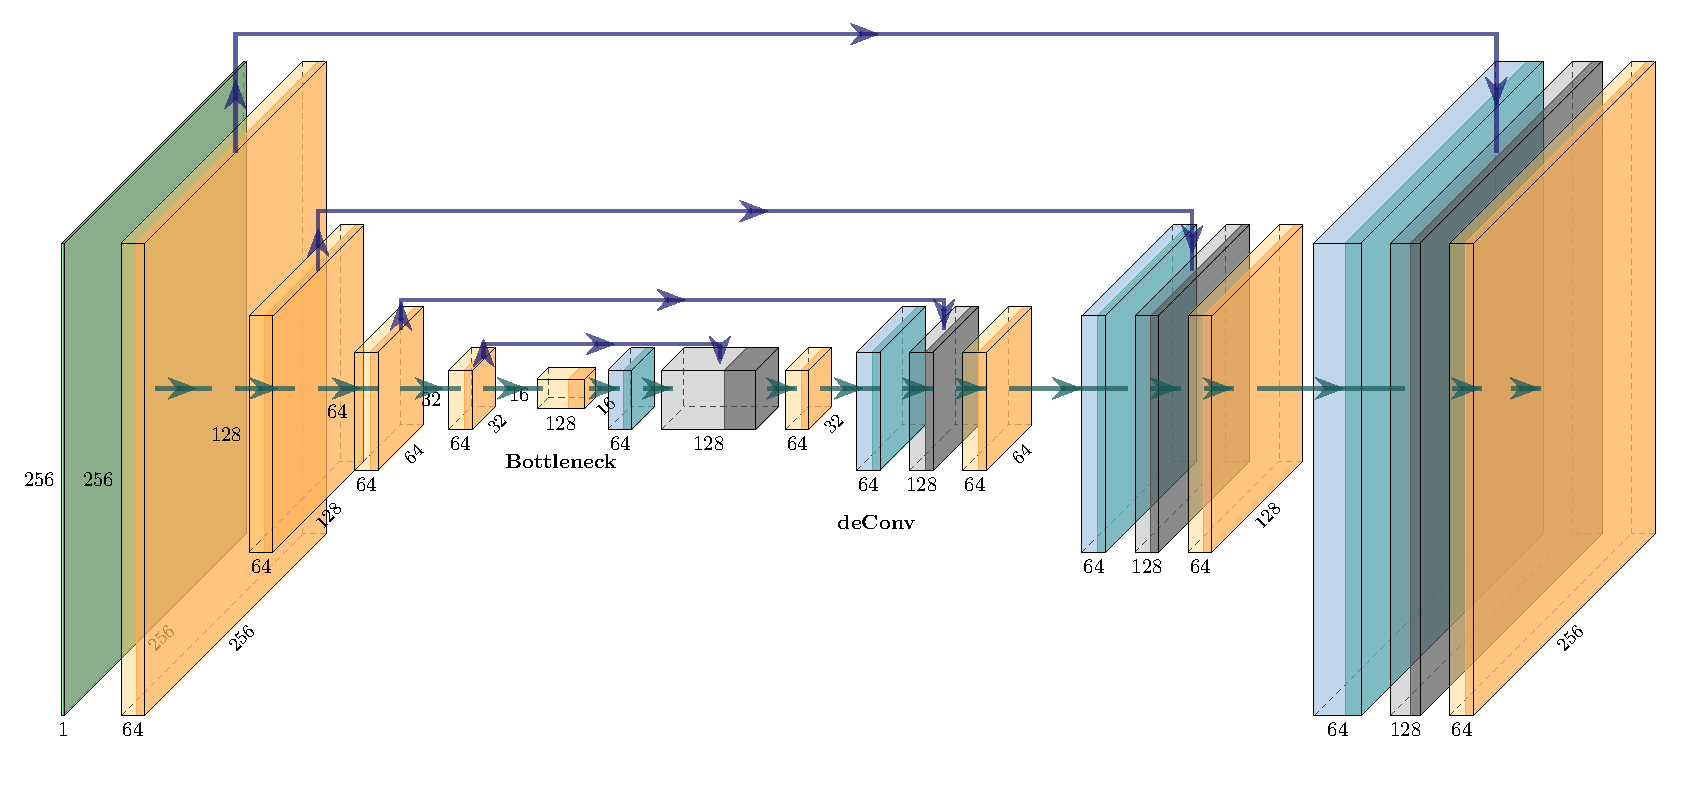
\includegraphics[scale=0.5]{figures/Unet}
	\caption{U-Net architecture used in this assignment.}
	\label{fig:U-Net1}
\end{figure}

\subsection{Network Design}
We design a U-Net-like architecture which is shown in Figure~\ref{fig:U-Net1}:
\begin{itemize}
	\item Use convolution with stride$=2$ for down-sampling and deconvolution for up-sampling. We also tried the combination of Max-Pooling and up-sampling. The experimental results show similar performance. The prior option is favored since convolution with stride$=2$ consumes less computational power than convolution with stride$=1$ and then pooling.
	\item Convolutions are done with the kernel size being $3\times 3$ and pad being $1$. Deconvolution are processed with the kernel size being $2\times 2$ and pad being 1.
	\item Dropout units are added before and after the bottleneck module.
\end{itemize}
We tried to implement the Mask R-CNN. However, the non-maximum suppression package doesn't match with the Pytorch version we are using, which make the compilation failure. 

\subsection{Data Preprocessing}
\subsubsection{Data Loading}
The dataset contains images of different size, which is not suitable for training. Two possible solutions could be use:
\begin{itemize}
	\item Similar to~\cite{ronneberger2015u}, we could pad image with constant value or with neighboring pixels for training. In this case, when testing, a sliding procedure is needed to process larger image. 
	\item Resize all images to a constant size.
\end{itemize}
Generally speaking, the first option is better than the second option since it doesn't loss any spatial information. However, it needs more workload. Because of the time limitation, we use the second option by resizing all images to $256\times 256$.
\subsubsection{Preprocessing} We convert image to gray scale image since it demonstates better performance, see Figure~\ref{fig:gray}. Besides gray scaling, we also tried several contrast enhancements since we found out that some images are low contrast. The results are shown in Figure~\ref{fig:prep}. The improvements are slight, thus finally we use simple gray scaling without other image enhancement.
\begin{figure}[ht]
	\centering
	\setlength{\fboxrule}{0.0pt}
	\framebox{\parbox{1.8in}{
			\centering
			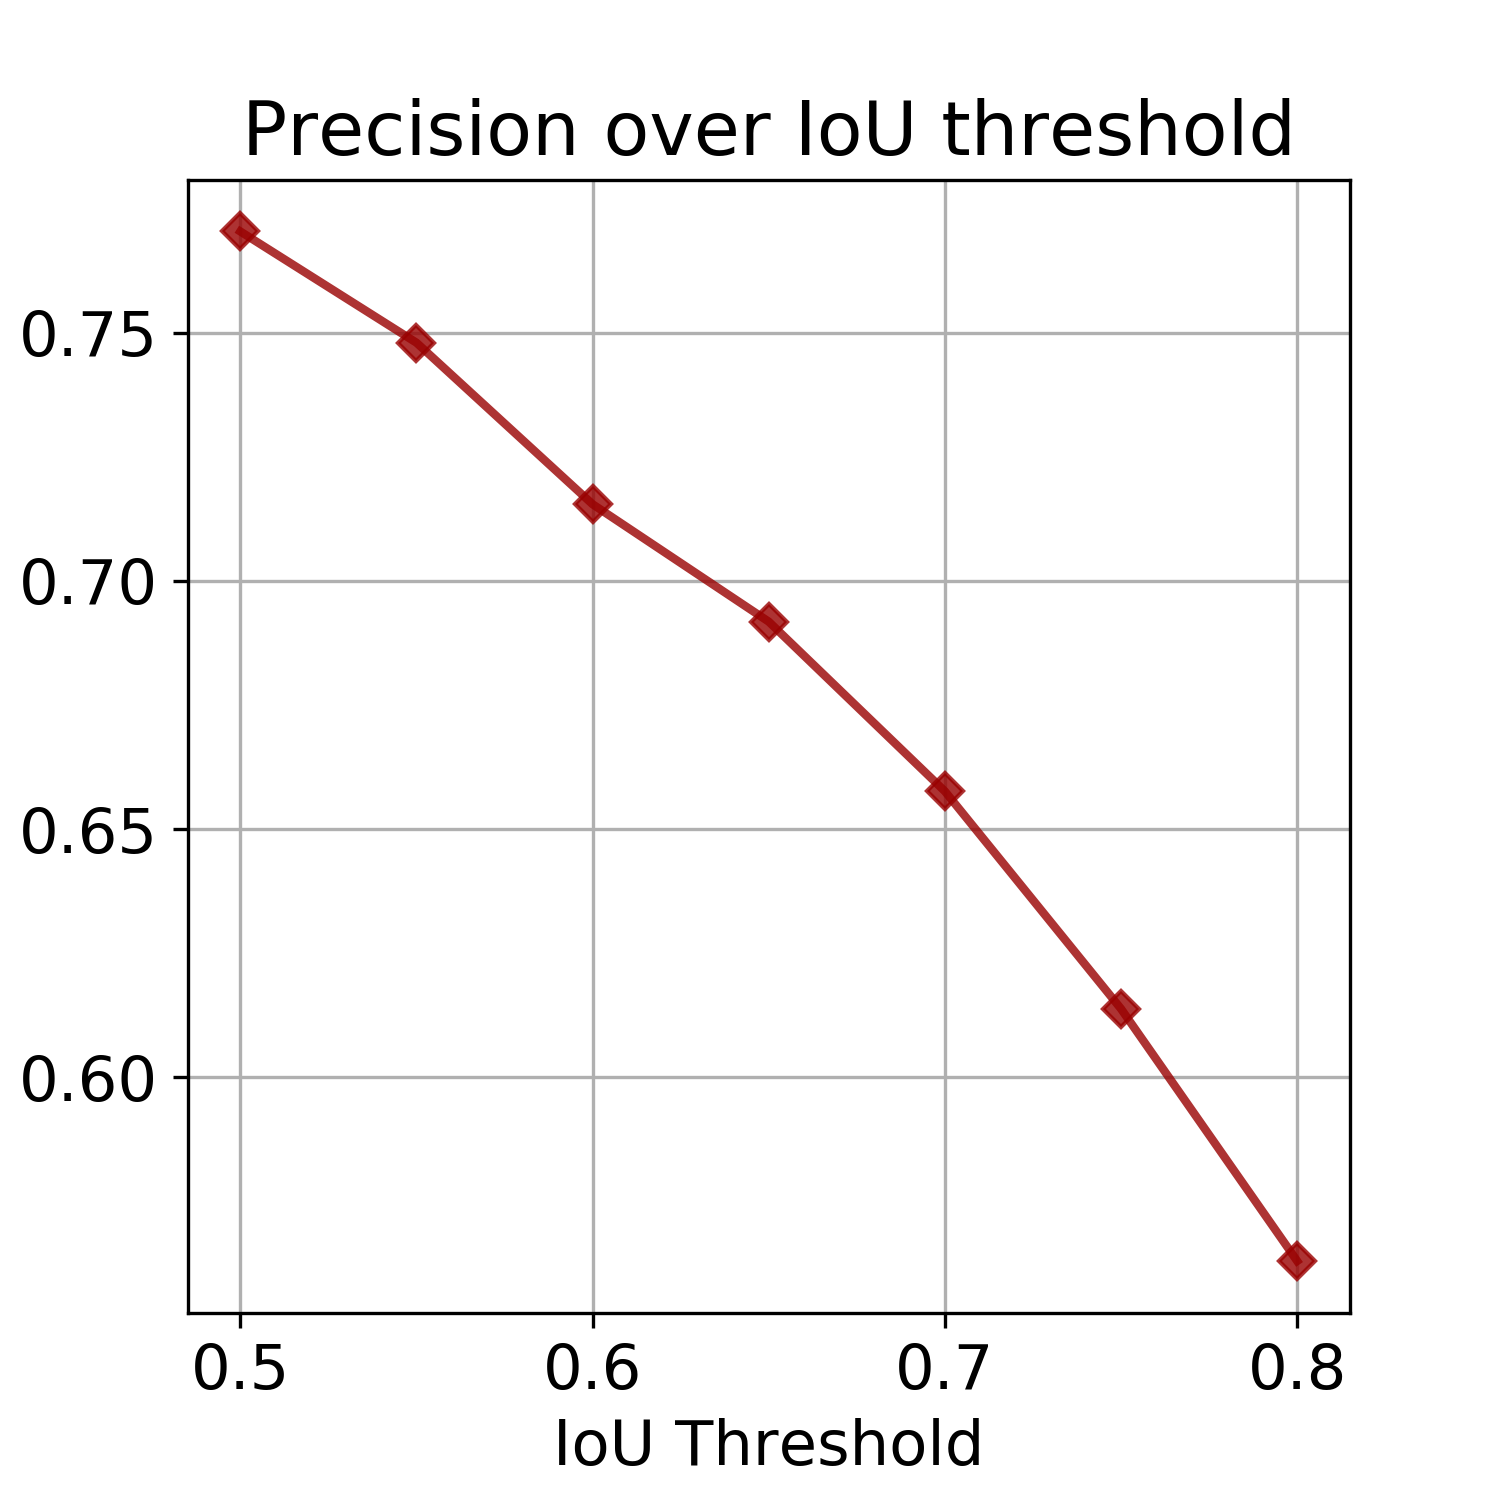
\includegraphics[width=5cm,height=5cm]{figures/prep/normal.png}
	}}
	\framebox{\parbox{1.8in}{
			\centering
			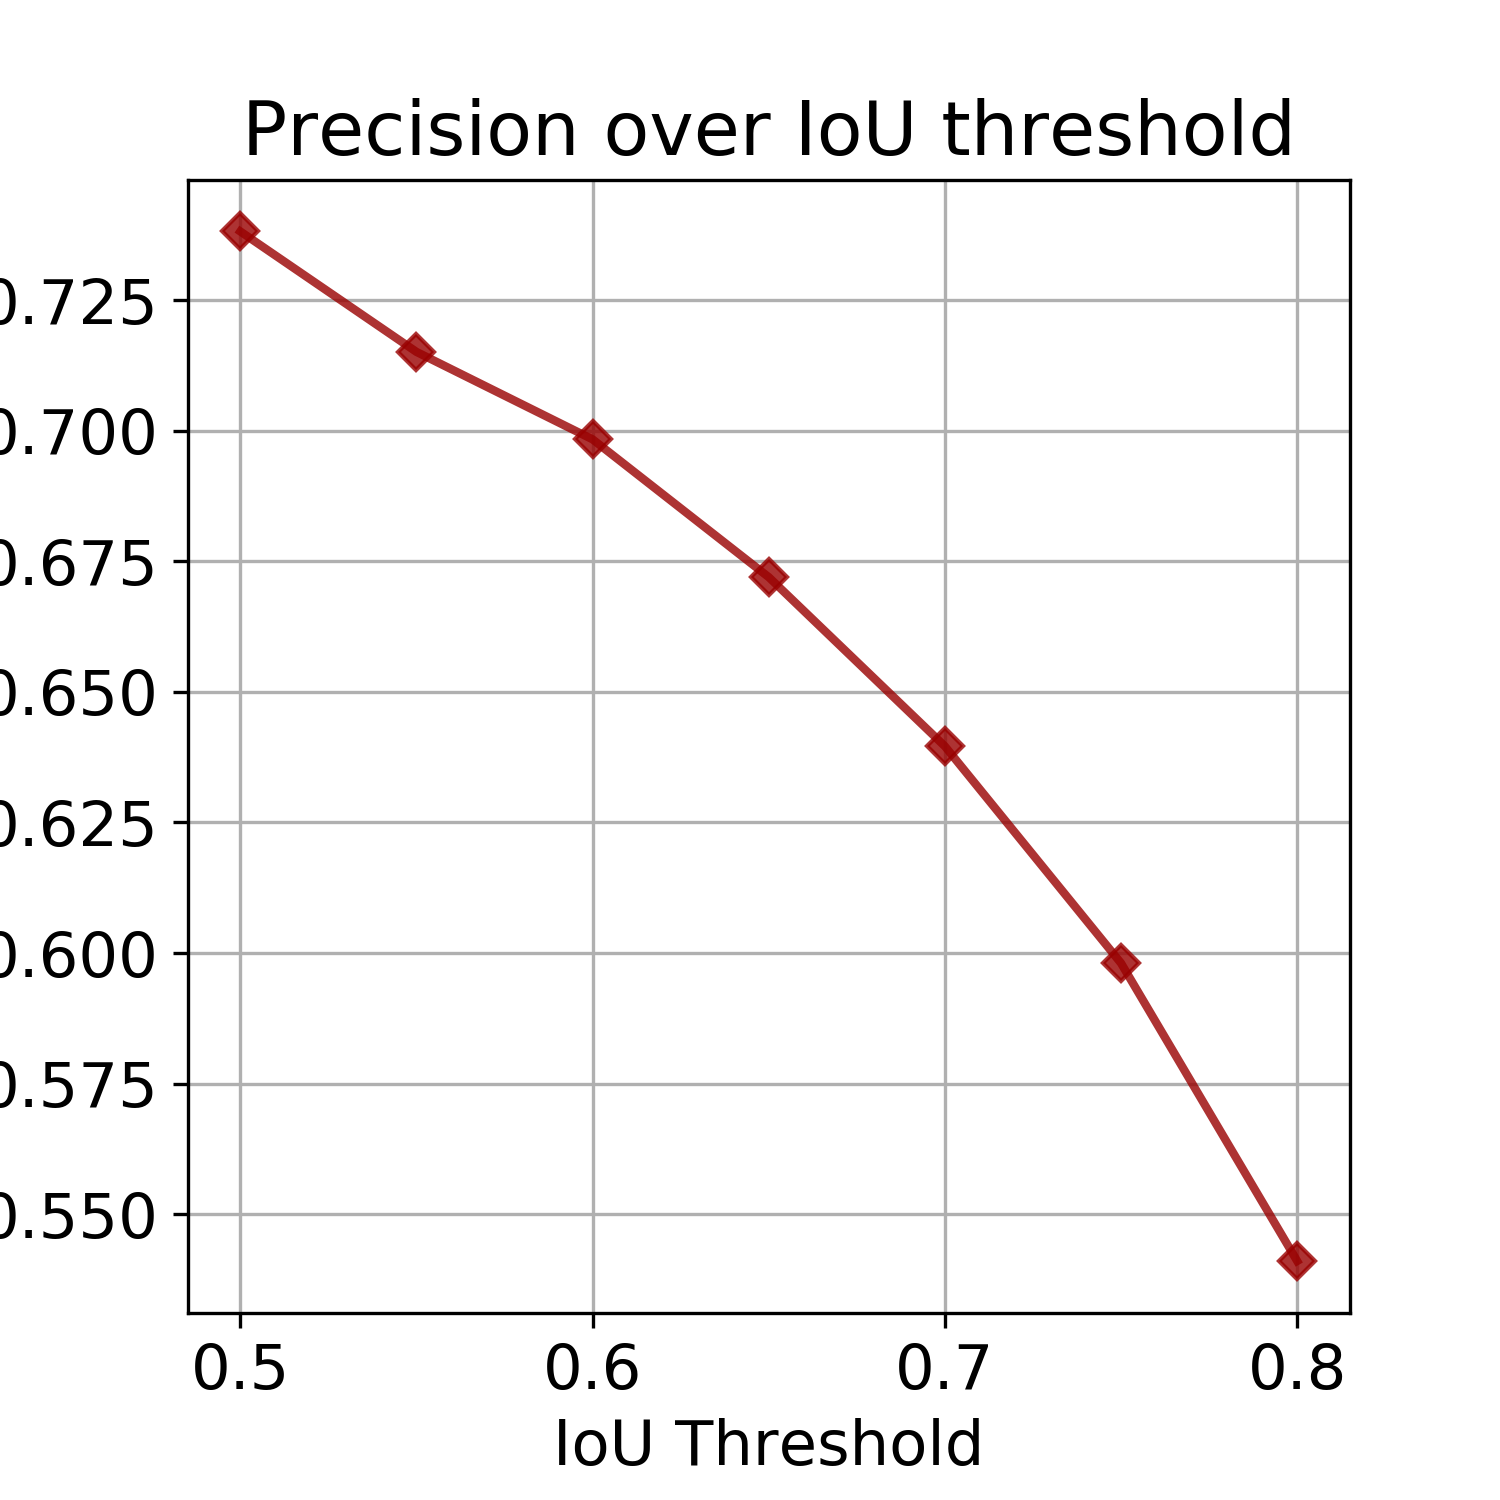
\includegraphics[width=5cm,height=5cm]{figures/prep/input_normalization_rgb.png}
	}} 
	\caption{Mean Average Precision over IoU threshold results: gray scale (left), RGB (right).}
	\label{fig:gray}
\end{figure}
\begin{figure}[ht]
	\centering
	\setlength{\fboxrule}{0.0pt}
	\framebox{\parbox{1.8in}{
			\centering
			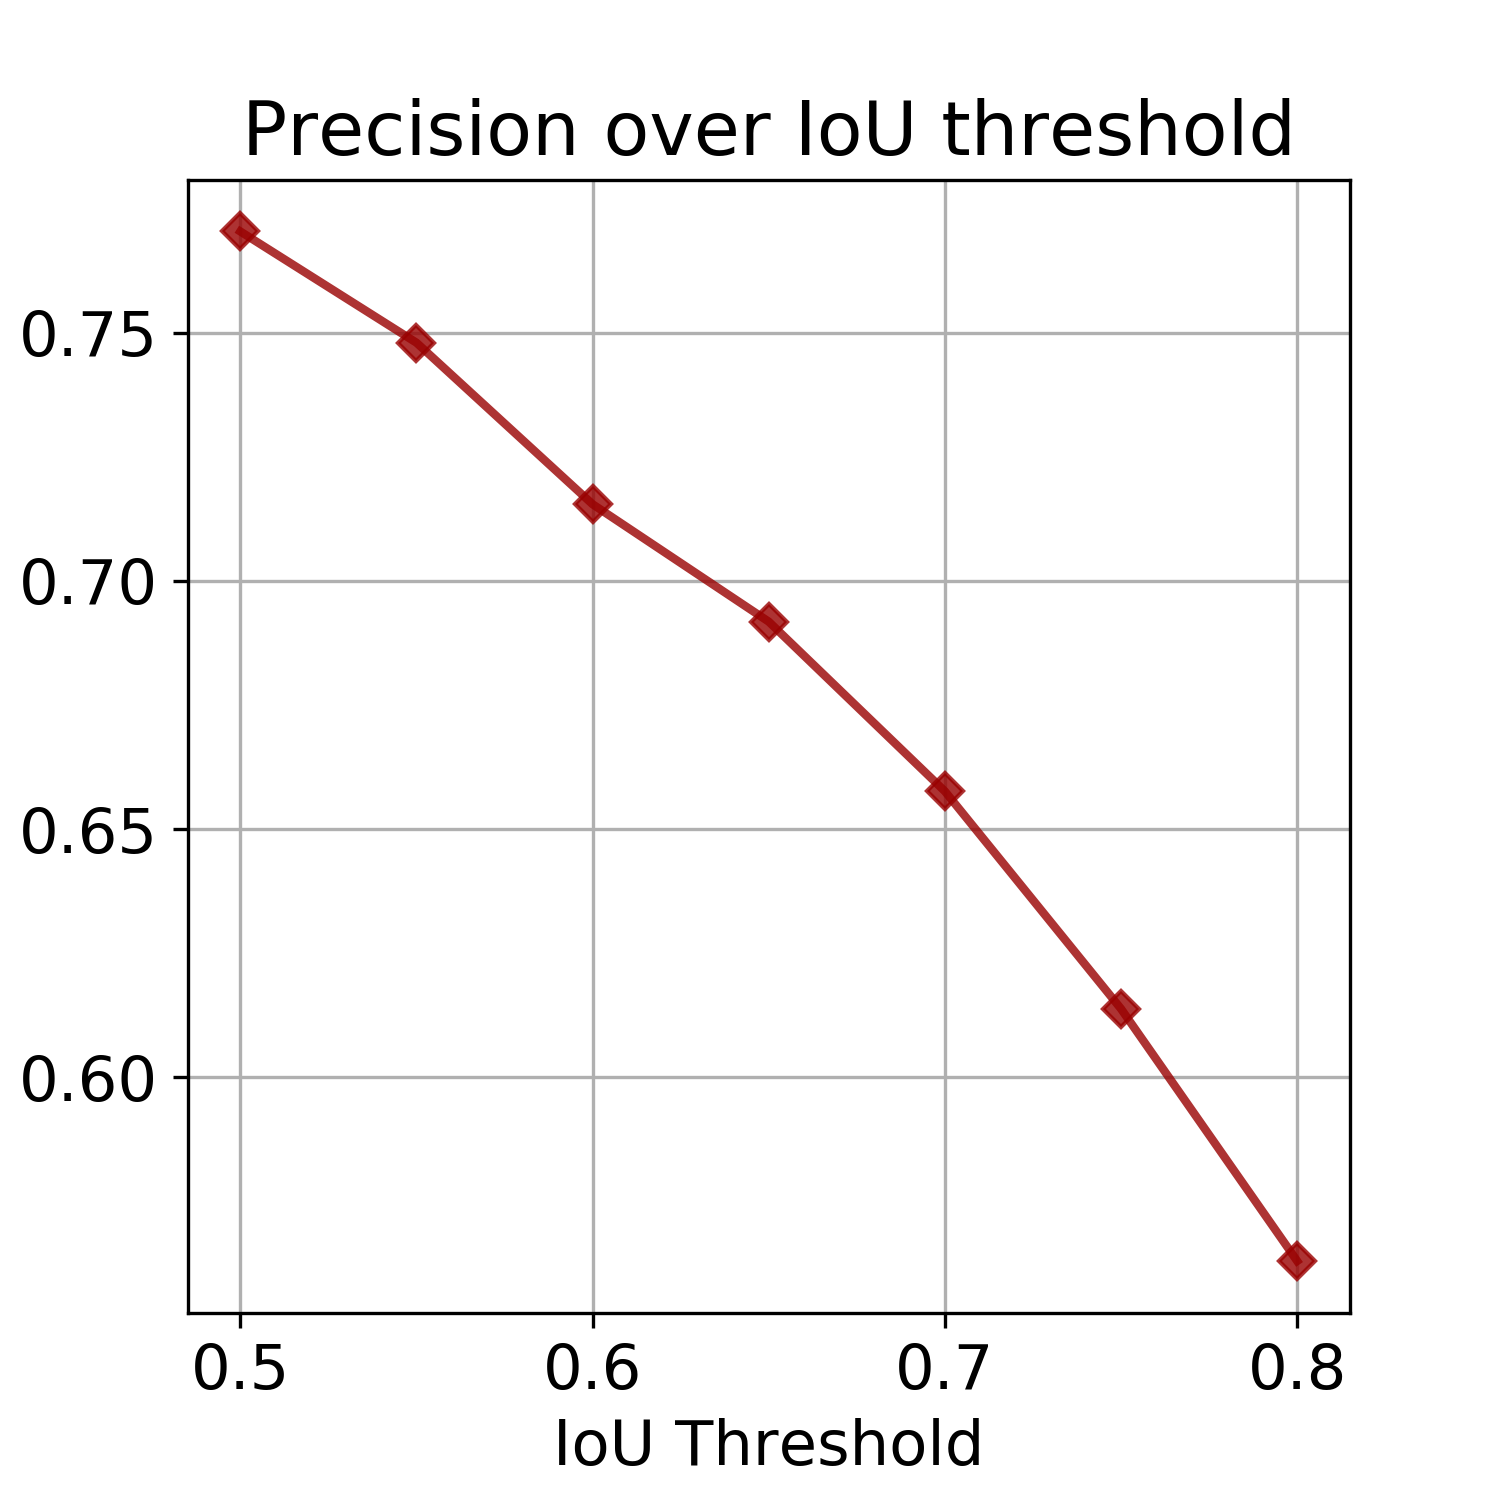
\includegraphics[width=5cm,height=5cm]{figures/prep/normal.png}
	}}
	\framebox{\parbox{1.8in}{
			\centering
			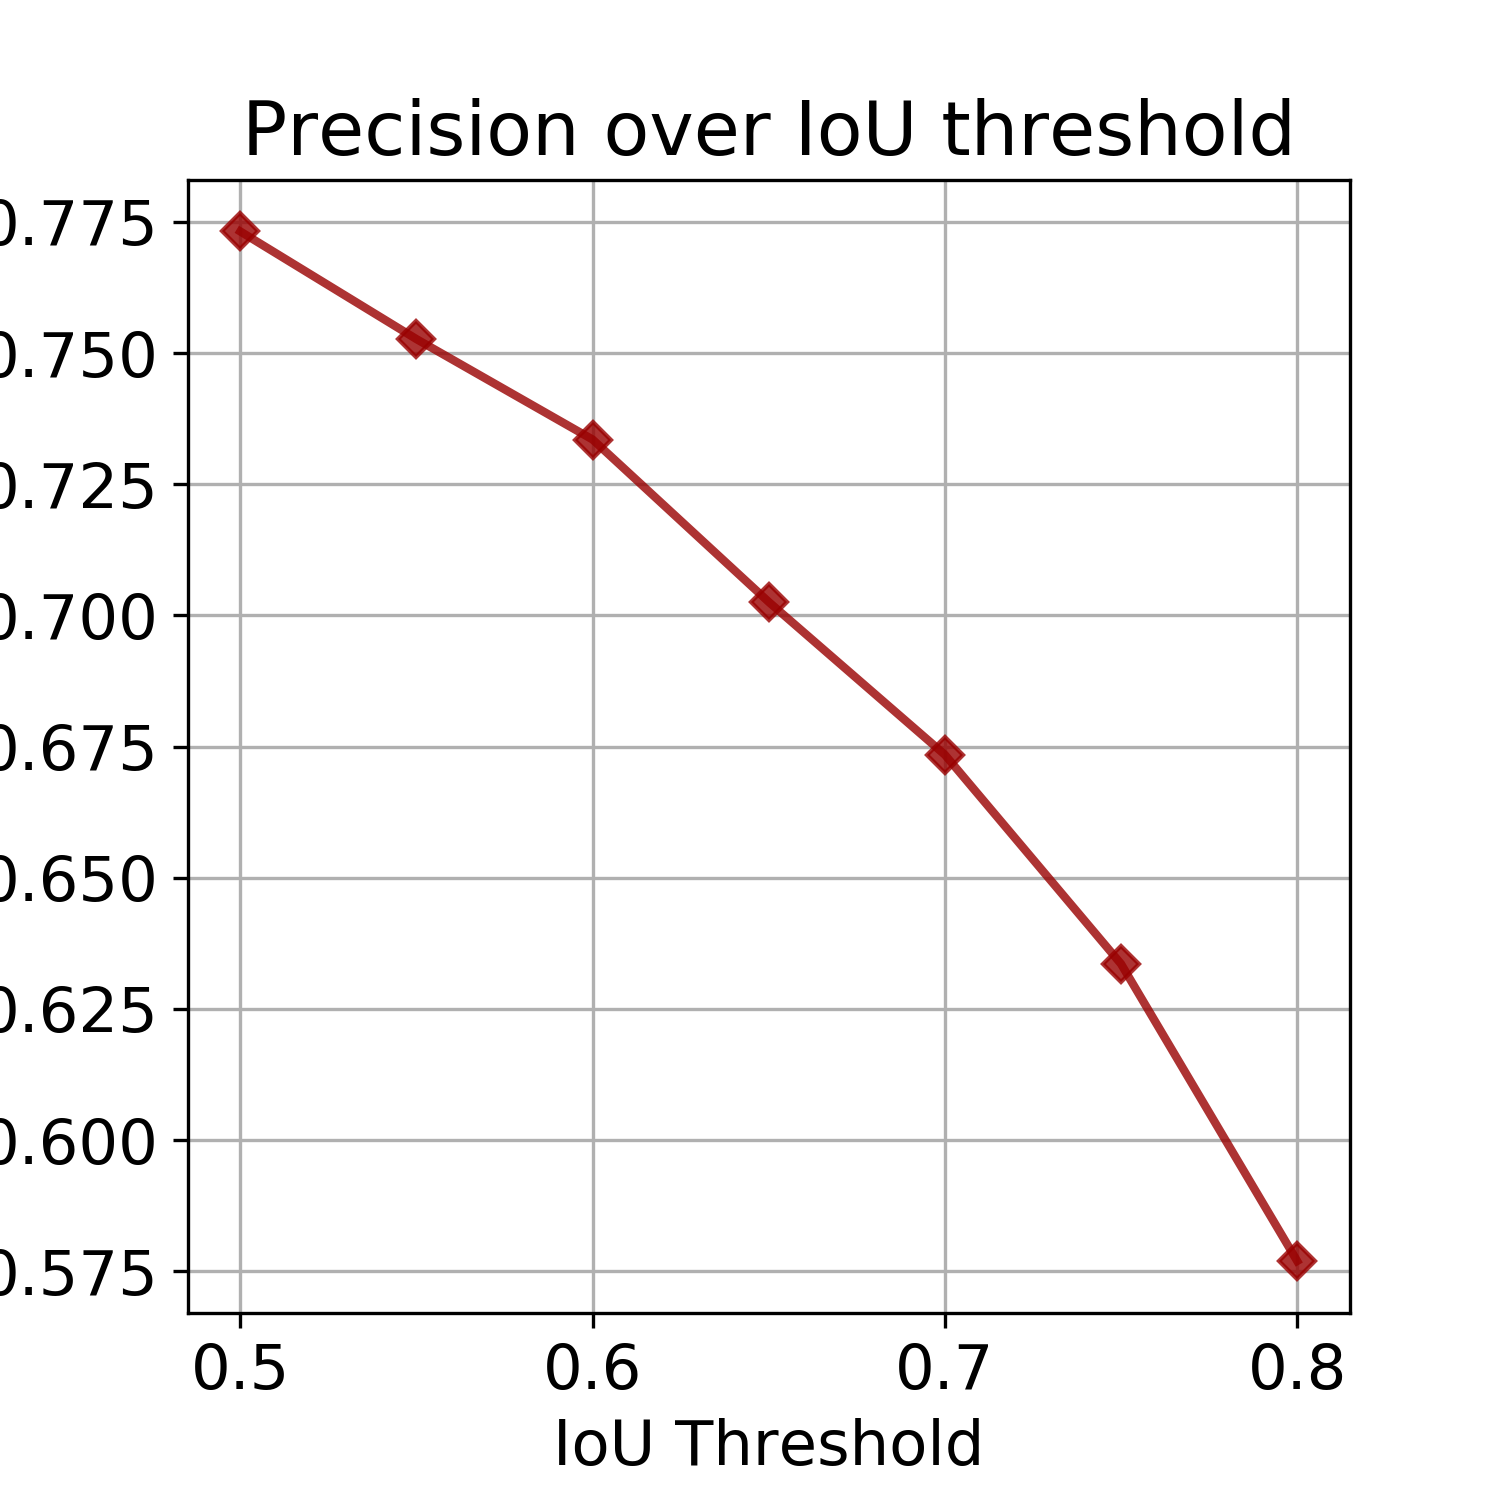
\includegraphics[width=5cm,height=5cm]{figures/prep/no_adjust_log.png}
	}} 
	\framebox{\parbox{1.8in}{
			\centering
			   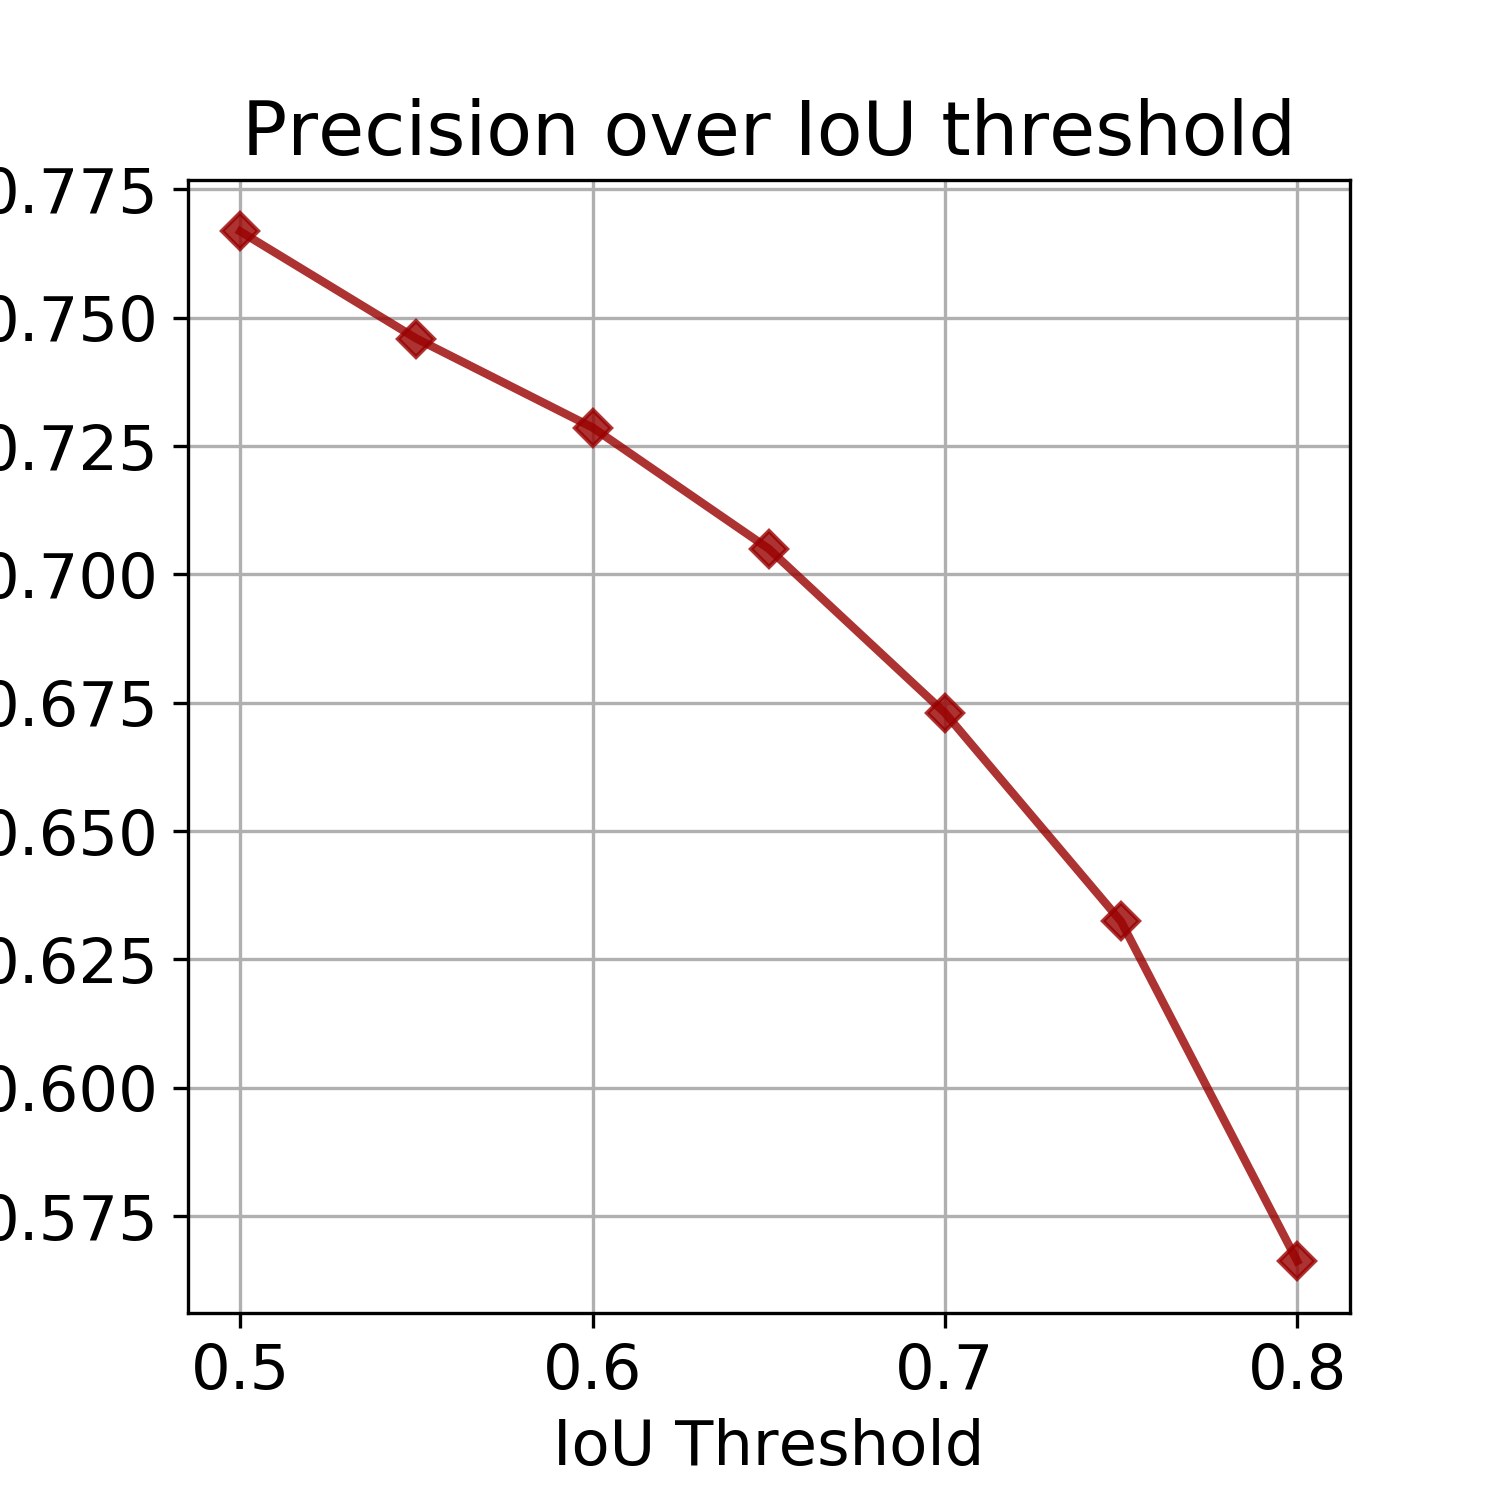
\includegraphics[width=5cm,height=5cm]{figures/prep/no_adjust_sigmoid.png}
	}}
	\caption{Mean Average Precision over IoU threshold results: Gray scale (left), Gray scale+logrithm correction (middle), and Gray scale + sigmoid correction (right).}
	\label{fig:prep}
\end{figure}
After gray images are obtained, we do input normalization to normalize the input to zero mean and standard deviation of $1$. 

\subsection{Post Processing}
After obtaining the predict feature map from U-Net, the sigmoid function is applied to get the probability map. By thresholding and extract component connected using watershed algorithm, all predicted nucleis can be indentified. \\
For evaluation, we do as follows:
\begin{enumerate}
	\item For all true masks, we use $\&$ binary operation to find its matched objects in the predicted map. If no match is found, then we add $1$ to the false negative.
	\item For matched objects, we select the one with biggest area and discard others. 
	\item Compute IoU using true mask and matched mask by $\&$ and $|$ binary operation.
	\item If IoU is over a threshold, then add $1$ to true positive and mask out matched mask in predicted map.
	\item After traversing all truth masks, false positive is counted as the remaining masks in the predicted map.
\end{enumerate}

\subsection{Further Improvement}
\subsubsection{Data Augmentation} Data augmentation for this task is more complex than the previous assignment since both image and mask need to be augmented. In order to support data augmentation, we divide data augmentation as \textbf{image transformation} and \textbf{geometric transformation}. Image transformation is only applied to raw image including constrast jetter, etc. Geometric transformation includes affine transformation (no shearing), resize, crop, etc. Detailed augmentation is shown as follows:
\begin{itemize}
    \item Affine transformation: rotation ($+/-\ 180$), translation ($+/-\ 0.01 \times {width, height}$), scaling ($0.8-1.2$). 
    \item RandomHorizontalFlip: flip in the horizontal way randomly (p=0.5).
	\item RandomVerticalFlip: flip in the vertical way randomly (p=0.5).
    \item Resize, rotate and center crop: resize to $350\times 350$, randomly rotate and then center crop the image to $256\times 256$.
\end{itemize}    
We finally took random horizontal and vertical flip as data augmentation.

\subsubsection{Erosion/Dilation}
After checking those worst segmentation images, we found out the major reason that the mean precision could not improve is because adjacent nucleis are segmented as a joint, which is even worse when large number of small nucleis are segmented as a big joint. In order to improve this case, we add erosion on the training masks to artificially segment close nucleis, while dilation is added at the end to compensate the side effect (thinner objects) of erosion. The gives us the best result on the validation data, as shown in the Figure~\ref{fig:erosion}.

\begin{figure}[ht]
	\centering
	\setlength{\fboxrule}{0.0pt}
	\framebox{\parbox{1.8in}{
			\centering
			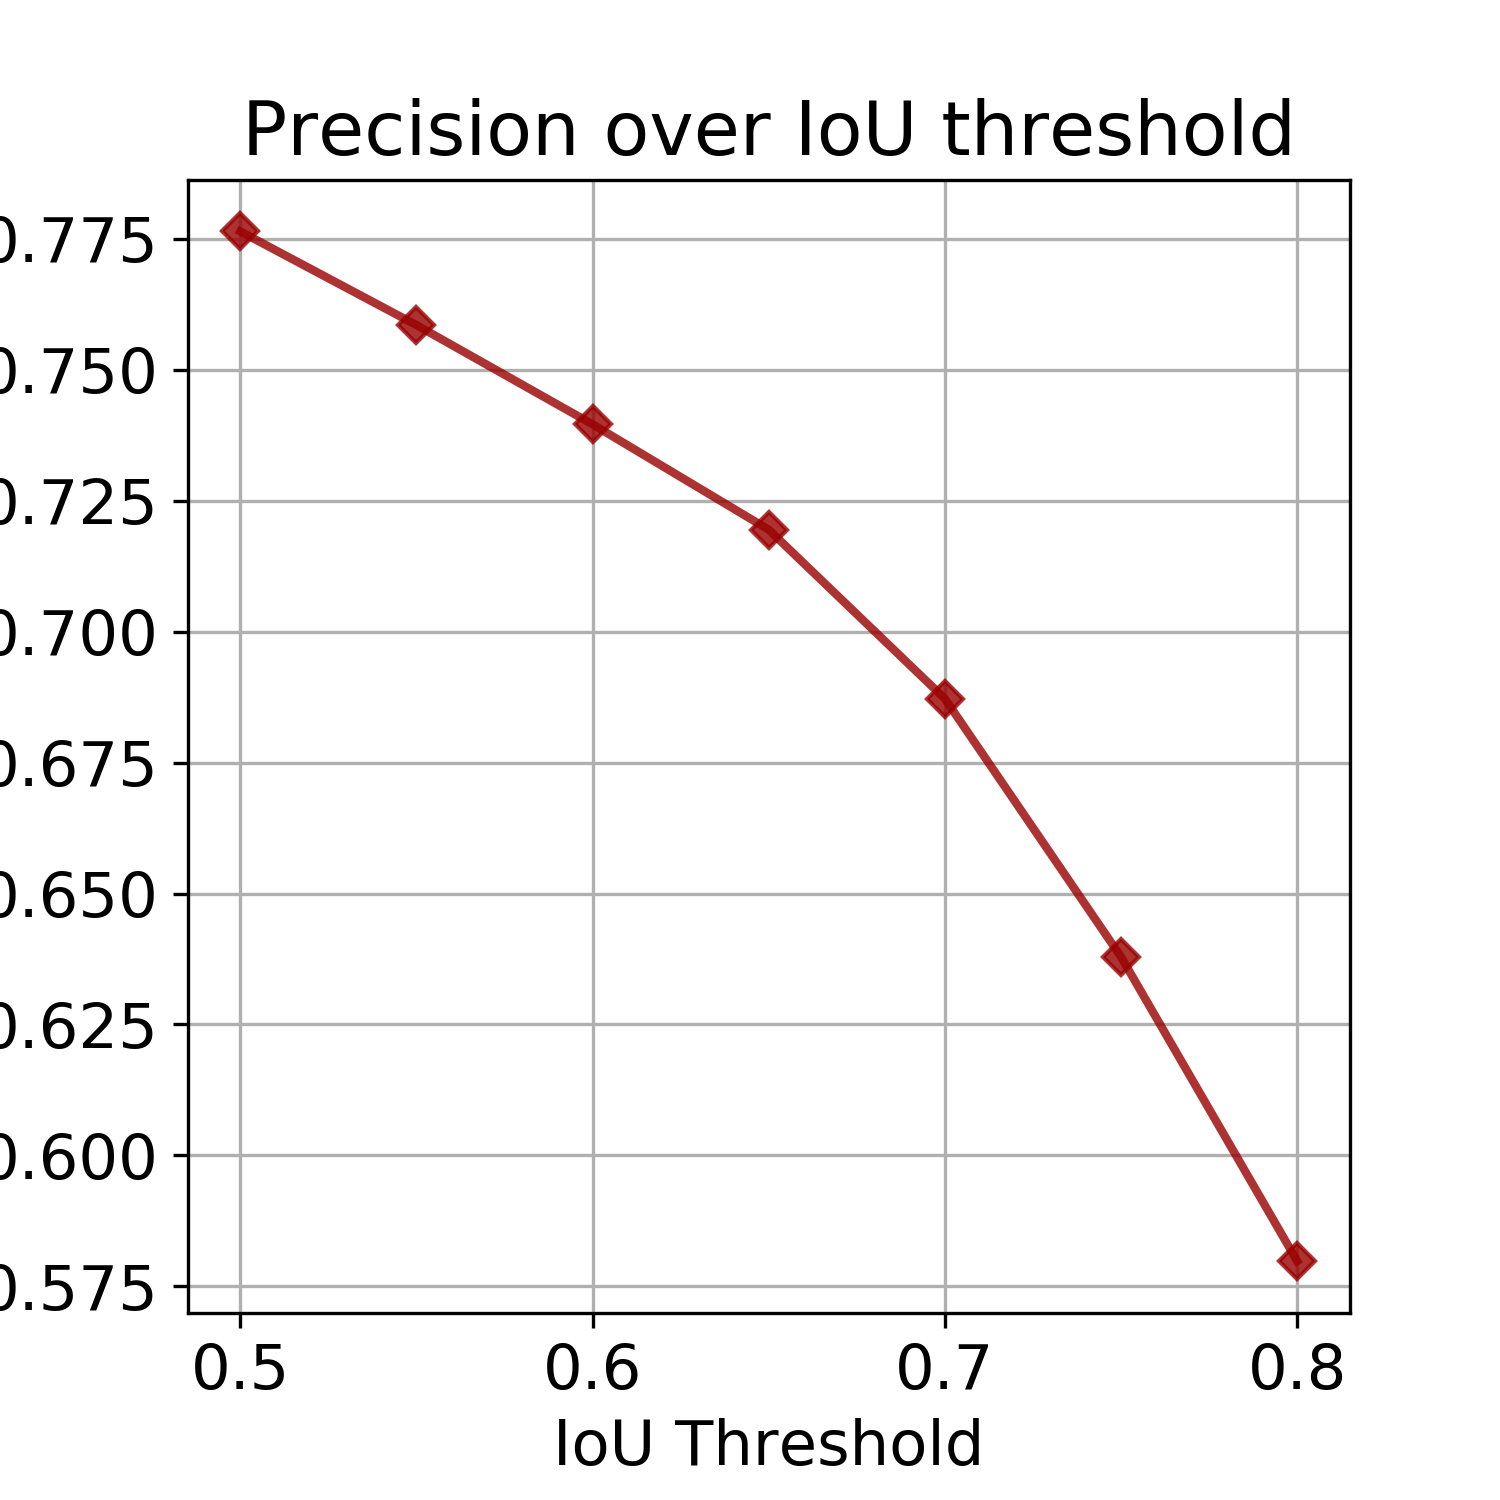
\includegraphics[width=5cm,height=5cm]{figures/prep/erosion_dilation_3x3.png}
	}}
	\framebox{\parbox{1.8in}{
			\centering
			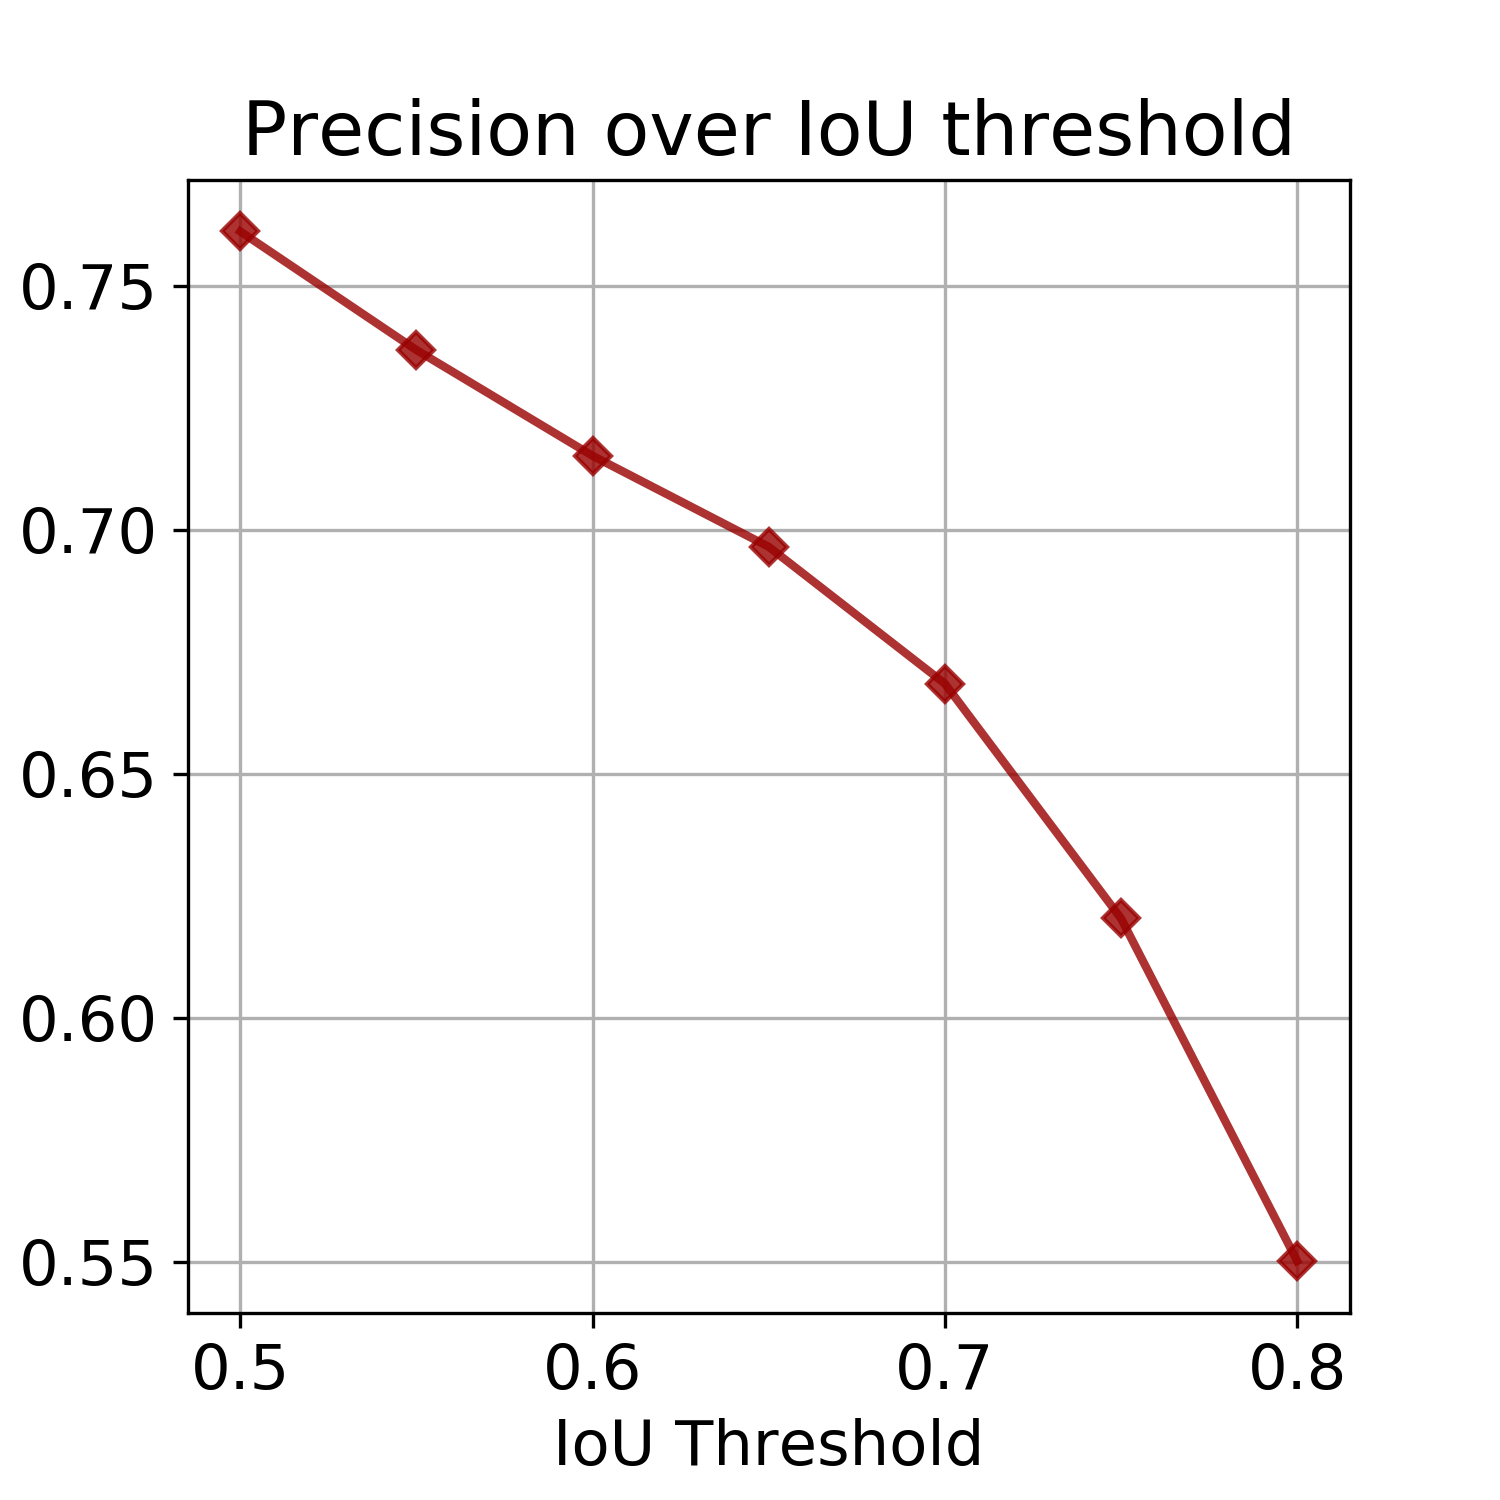
\includegraphics[width=5cm,height=5cm]{figures/prep/erosion_dilation_5x5.png}
	}} 
	\caption{Mean Average Precision over IoU threshold results with erosion/dialation using square mask: mask size ($3\times 3$) (left), mask size ($5\times 5$)  (right).}
	\label{fig:erosion}
\end{figure}

\subsubsection{Use Contour} We tried to add contour as the third class, which aims to better seperate close nucleis:
\begin{enumerate}
	\item Find contour on the training masks and label those pixels as border class.
	\item Rewrite loss function using softmax since we are dealing with three class classification problem.
	\item When doing instance segmentation, firstly treate border pixels as foreground pixels and segment. After that, we check if a border pixel is inside a segment (check if 4-neighbors are all masked pixels). We then delete those border pixels inside the segment.
\end{enumerate}
Since border pixels inside an image is much less than other pixels, for class balance, we create weights using the inverse frequency of each class as:
$$
weight_i = \frac{\sum_{N,H,W}1}{\sum_{N,H,W}l==i},\ \ i=1,\ 2,\ 3
$$
Weights will further be normalized with their sum being $1$.\\
Because of time limitation, we haven't thoroughly completed this improvement (step $3$). We tried to process with the intermediate results, but the performance was not very promissing.


%
%\begin{table}[]
%\centering
%\caption{Optimizer Analysis: $lr=1e-4$ and $epoch=15$\label{Op_Ana}}
%\scalebox{0.9}{
%\begin{tabular}{|c|c|c|c|c|}
%\hline
%\textbf{Optimizer Type}    & \textbf{Train Accuracy} & \textbf{Test Accuracy} & \textbf{Spending Time} & \textbf{Epochs at convergence} \\ \hline
%\textbf{SGD}               & 88.4\%                  & 90.9\%                 & 4:31                   & 30                             \\ \hline
%\textbf{SGD with Momentum} & 92.3\%                  & 93.1\%                 & 4:36                   & 25                             \\ \hline
%\textbf{Adam}              & 96.9\%                  & 93.9\%                 & 4:54                   & 15                             \\ \hline
%\textbf{RMSProp}           & 95.8\%                  & 93.1\%                 & 4:49                   & 15                             \\ \hline
%\end{tabular}}
%\end{table}

\begin{figure}[ht]
	\centering
	\setlength{\fboxrule}{0.0pt}
	\framebox{\parbox{2.5in}{
			\centering
			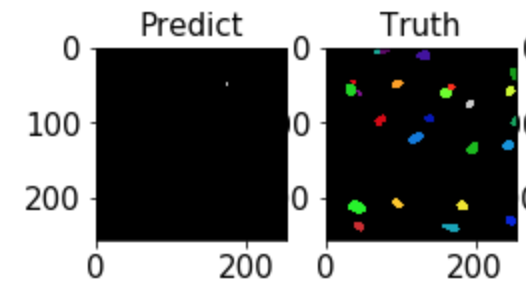
\includegraphics[width=5cm,height=5cm]{figures/prep/good1.png}\\
			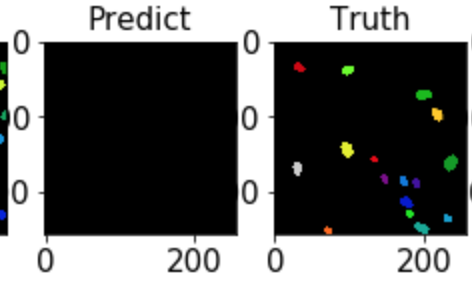
\includegraphics[width=5cm,height=5cm]{figures/prep/good2.png}\\
			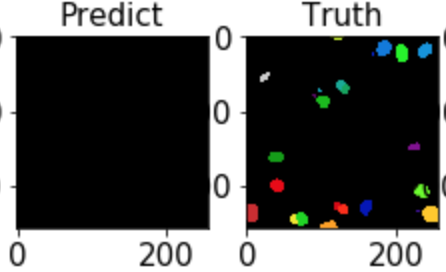
\includegraphics[width=5cm,height=5cm]{figures/prep/good3.png}
	}}
	\framebox{\parbox{2.5in}{
			\centering
			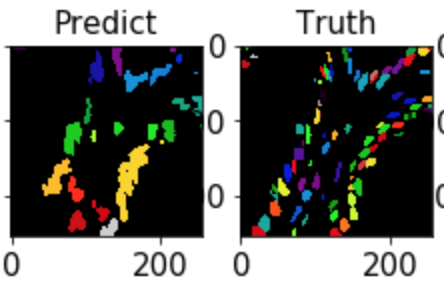
\includegraphics[width=5cm,height=5cm]{figures/prep/bad1.png}\\
			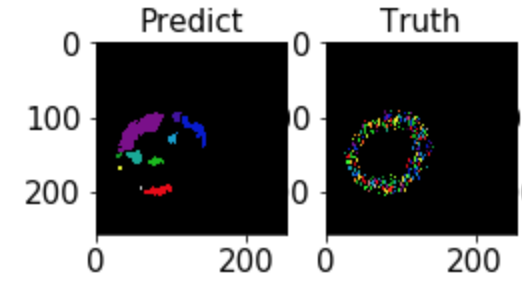
\includegraphics[width=5cm,height=5cm]{figures/prep/bad2.png}\\
			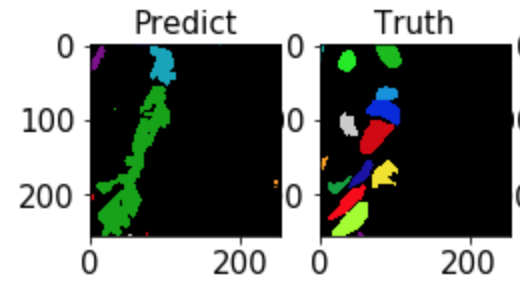
\includegraphics[width=5cm,height=5cm]{figures/prep/bad3.png}
	}} 
	\caption{Segmentation results: good (left), bad (right). Illustration of figures: since we will remove masks in the predicted map if a corresponding unique nuclei in true mask can be found, so for good results, you will see the predicted map as a blank image (all masks have been removed).}
	\label{fig:res1}
\end{figure}
\begin{figure}[ht]
	\centering
	\setlength{\fboxrule}{0.0pt}
	\framebox{\parbox{5.8inn}{
			\centering
			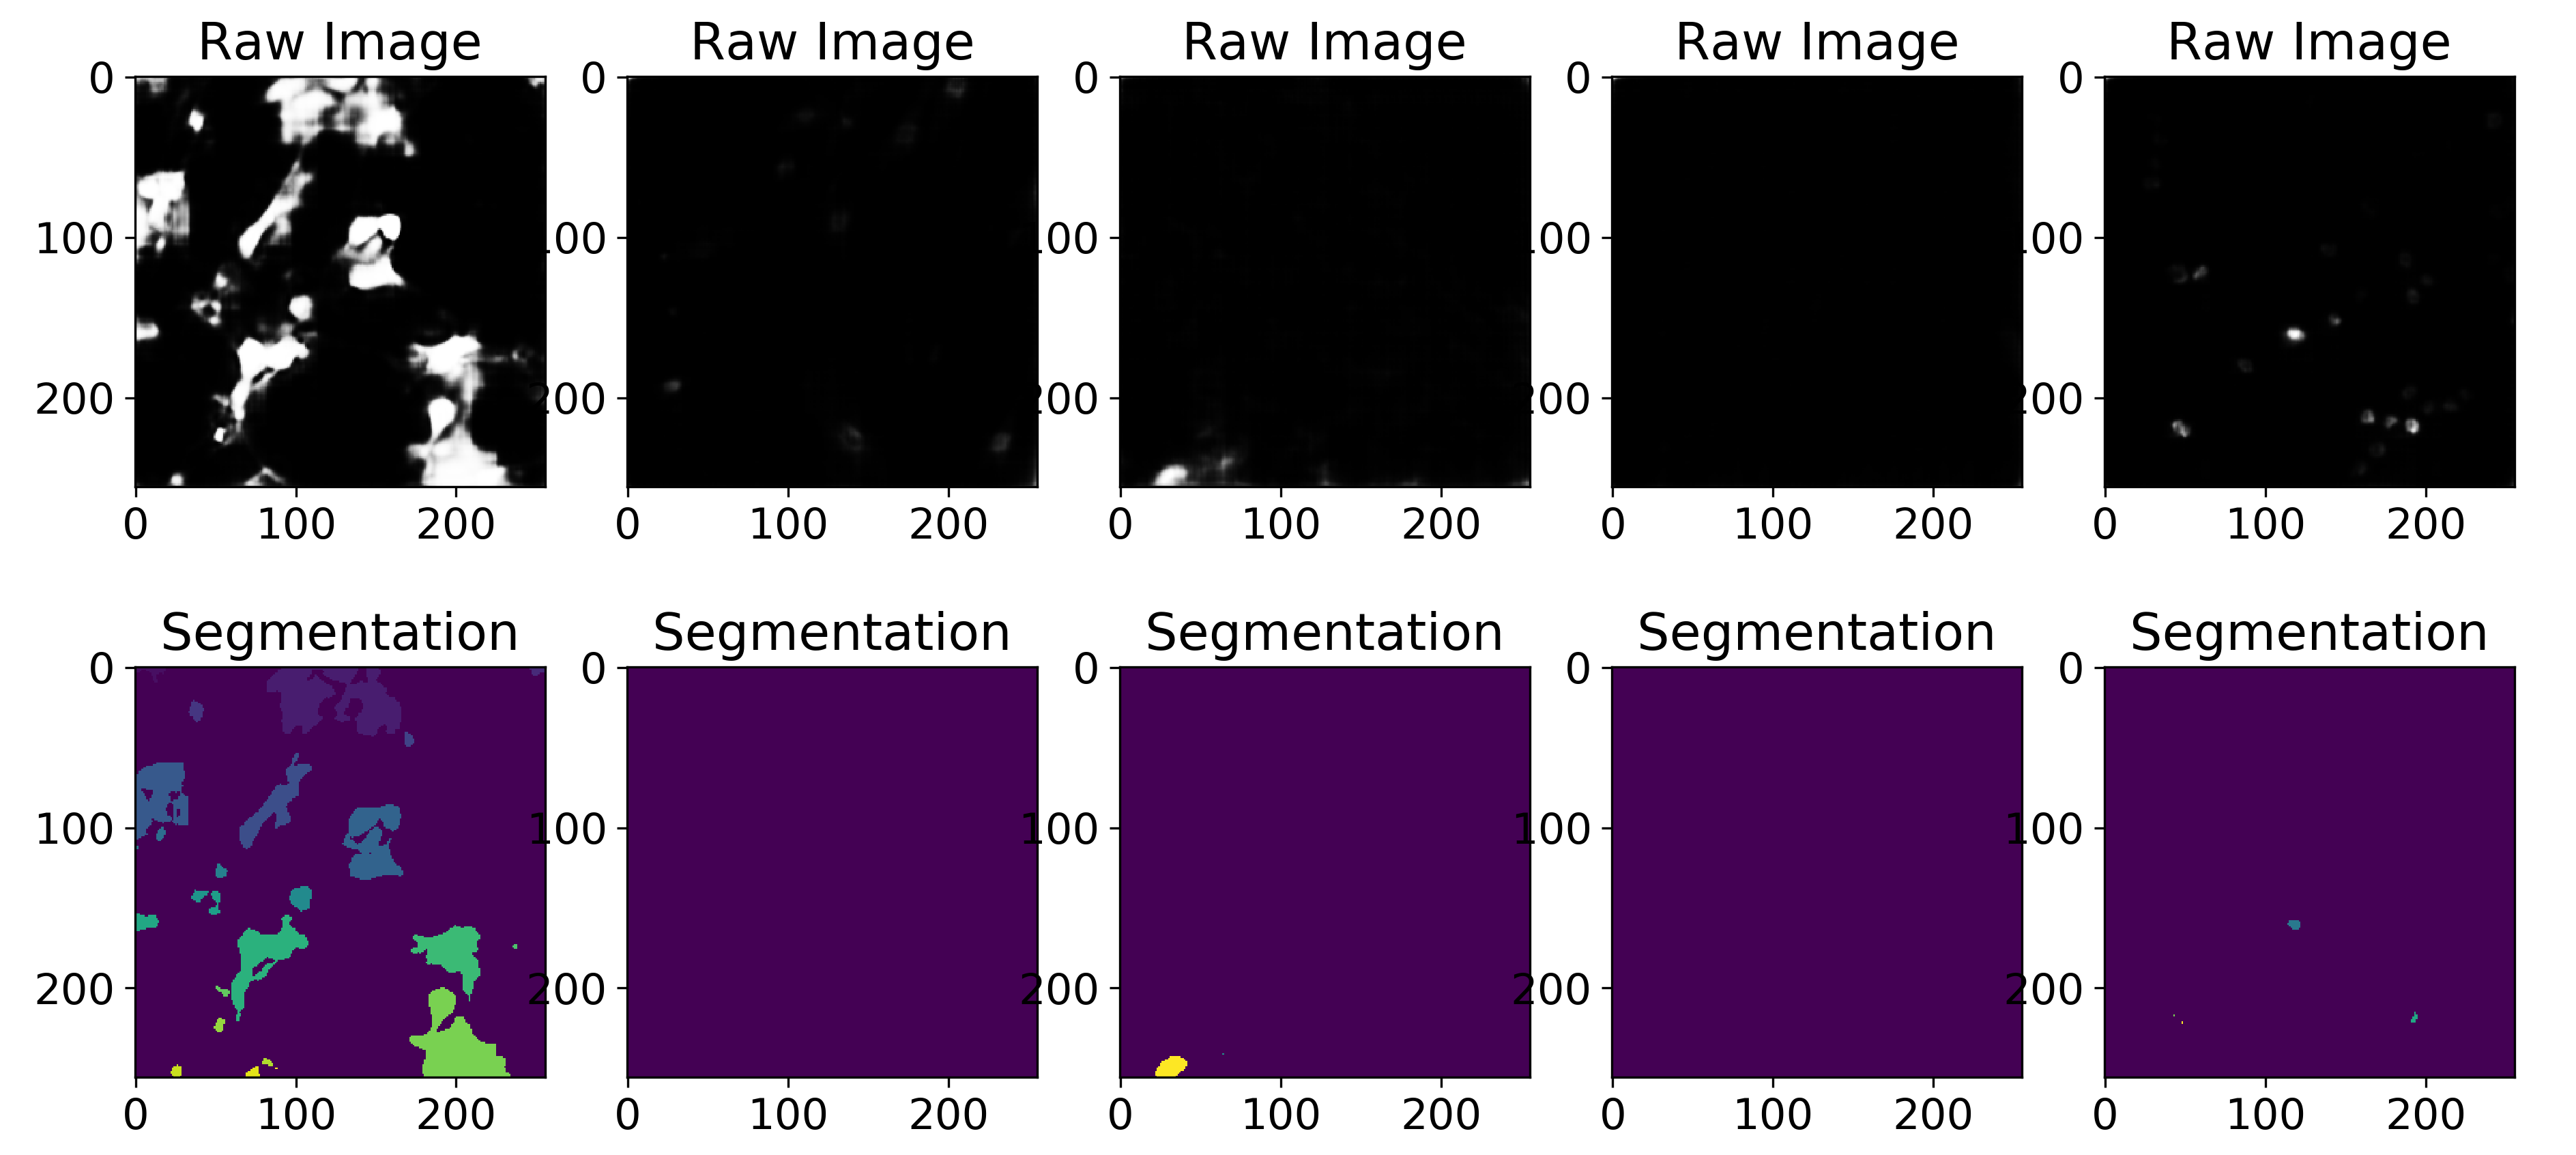
\includegraphics[width=\textwidth]{figures/prep/test_result_on_segment.png}
			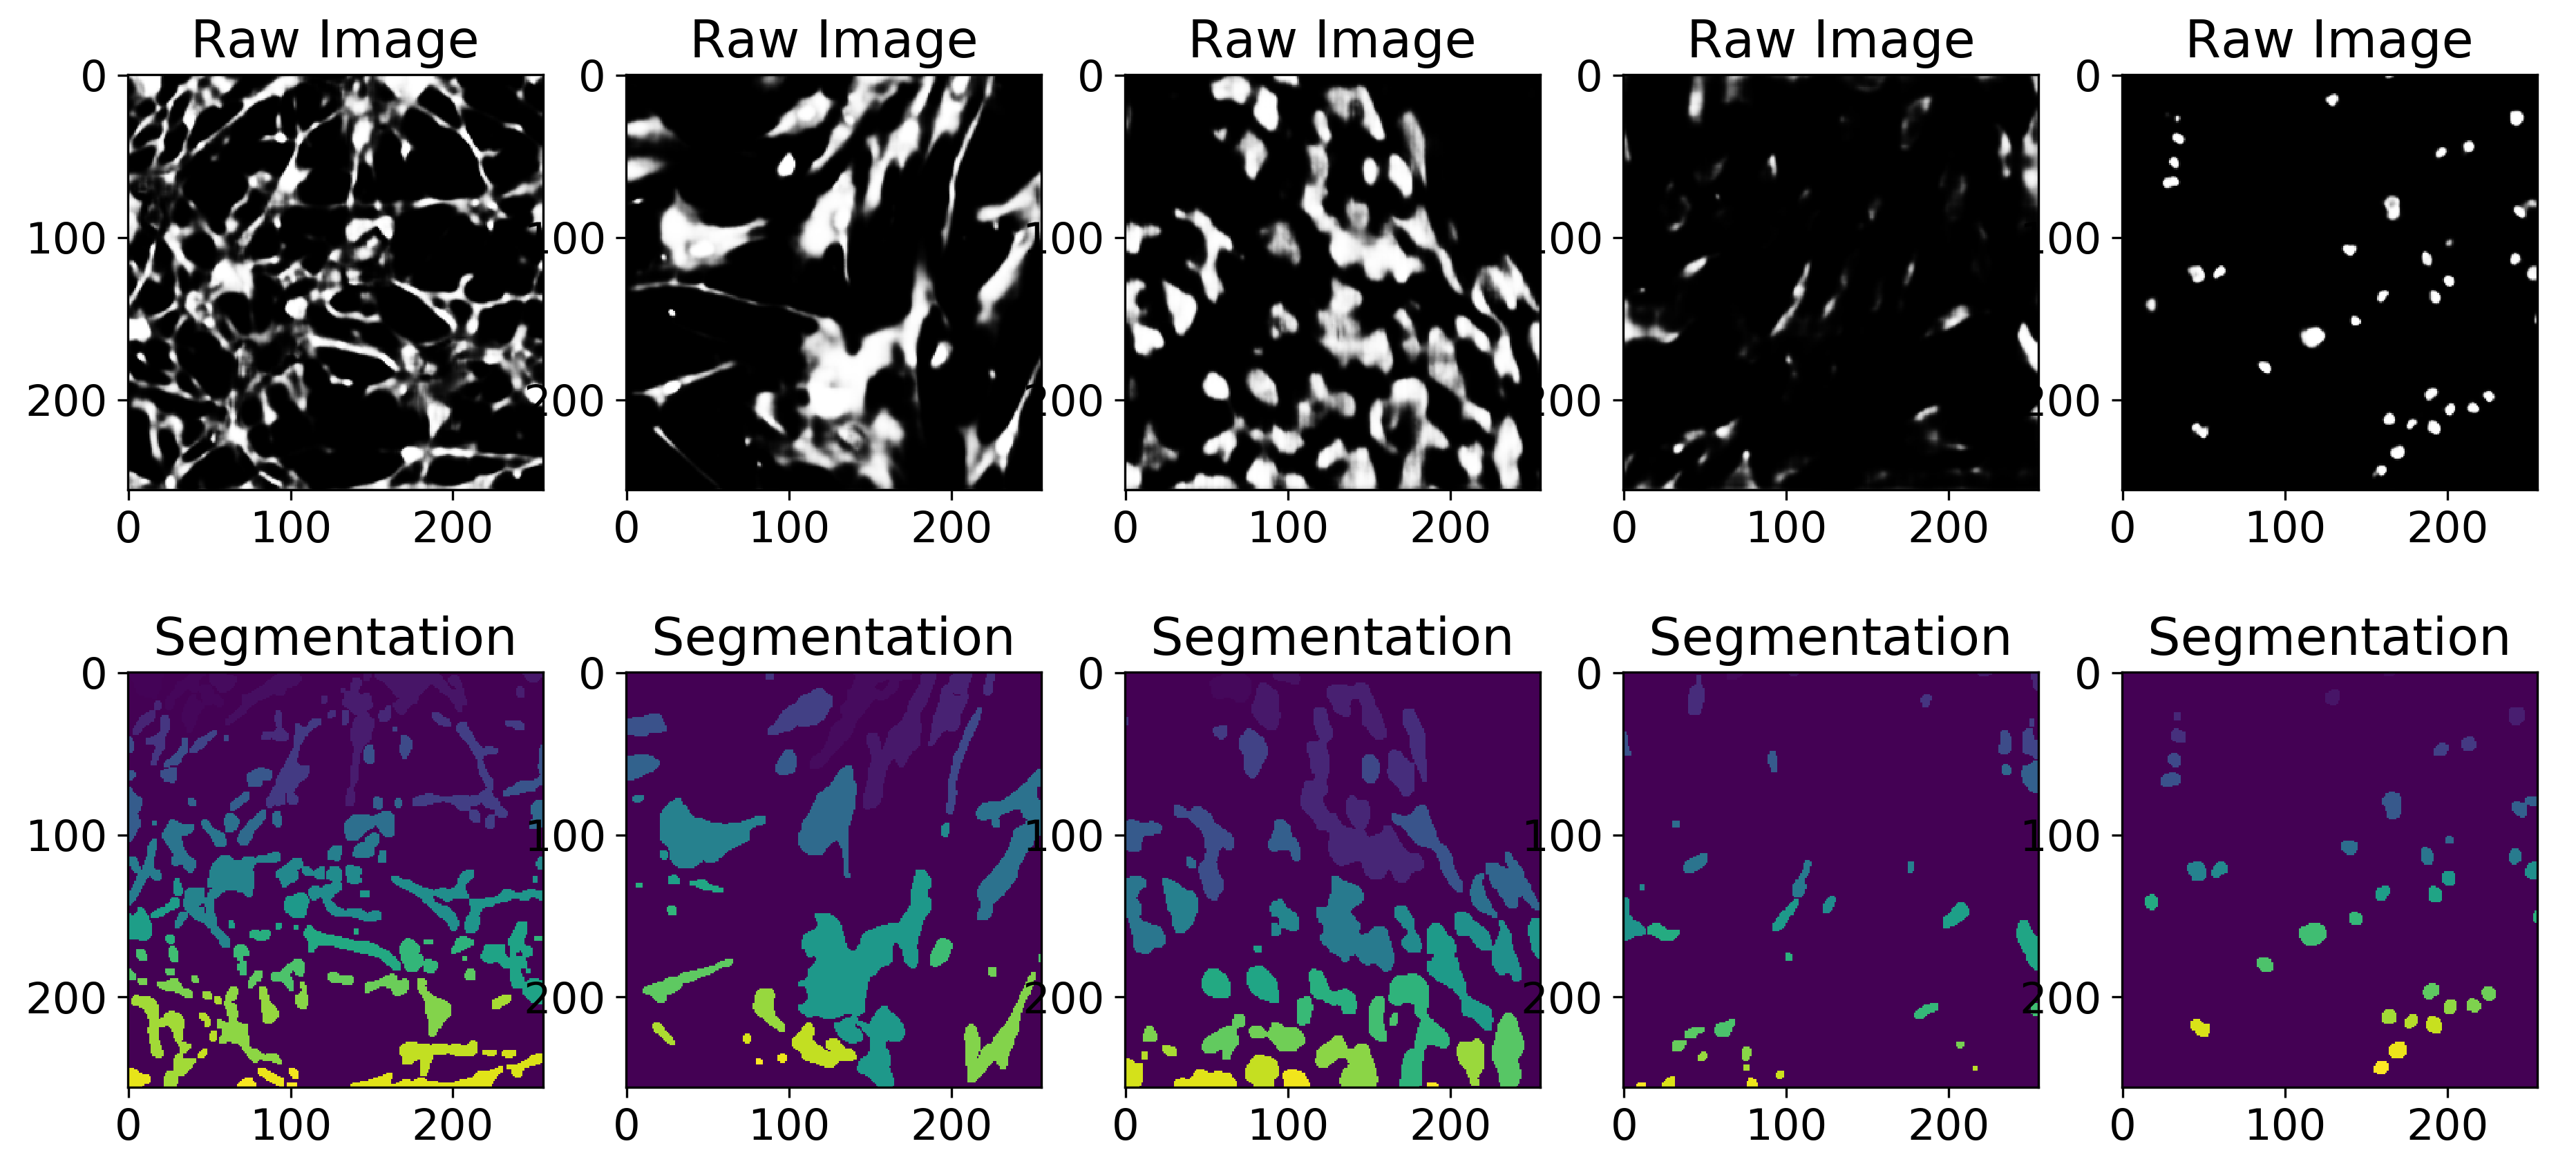
\includegraphics[width=1\textwidth]{figures/prep/test_result_on_segment_normal.png}
			\caption{Segmentation results on stage 2 images: top (with input normalization), bottom (without input normalization).}
	}}
	\label{fig:res2}
\end{figure}

\subsection{Result \& Analysis}
The mean average precision over IoU threshold is shown in Figure~\ref{fig:erosion}. It drops from $\approx 77\%$ when IoU threshold is $0.5$ to $\approx 59\%$ when IoU is $0.8$. Some segmentation results are shown in Figure~\ref{fig:res1}. It can be seen that for nucleis with sufficient margin, the network can segment them very well. However, the real challenging part is the case where large number of nucleis are close to each other.

Figure~\ref{fig:res2} shows the result on stage 2 test images provided by the instructor. It can be seen input normalization severely change the appearance of the input images and make the segmentation worse than that without input normalization. It can be concluded that input normalization should be done in a proper way with regarding to the data at hand.

Several points need to be considered for future improvement:
\begin{itemize}
	\item Use advanced region proposal network like the one in Faster R-CNN for better segmenting close objects.
	\item Proper way of doing data augmentation and input normalization for a specific task.
\end{itemize}

%
%\begin{subappendices}
%	\renewcommand{\thesection}{\Alph{section}}%
%	\subsubsection{Loss Function} We applied several loss functions to the training. 
%	\\BCE:
%	\begin{equation}
%	L_{BCE}=\hat{y}-y\hat{y}+log(1+exp(-\hat{y}))
%	\end{equation}
%	Dice loss:
%	\begin{equation}
%	L_D(X,Y)=1-\frac{1}{256\times 256}\sum_i\frac{2X_i\times Y_i}{X_i+Y_i}
%	\end{equation}
%	Focal loss:
%	\begin{equation}
%	L_{focal}(y,\hat{y})=-\sum_i\Bigg[(1-\sigma(\hat{y_i}))^\gamma y_ilog\sigma(\hat{y_i})+(1-y_i)log(1-\sigma(\hat{y_i}))\Bigg]
%	\end{equation}
%	BCE with regularization
%	\begin{equation}
%	L_{contiguity}=\sum_{i,j}|\sigma(\hat{y_{i+1,j}}-\sigma(\hat{y_{i,j}})|+\sum_{i,j}|\sigma(\hat{y_{i,j+1}}-\sigma(\hat{y_{i,j}})|)
%	\end{equation}
%	According to the result we get, the dice loss function gets the best training image, and also it learns faster than the focal loss.
%	The trianing and test results are as follows:
%	%%%%%%%%%%%%figure 2
%	\begin{figure}[H]
%		\centering
%		%    \subfig{
%		\label{Fig_bce3.sub.1} 
%		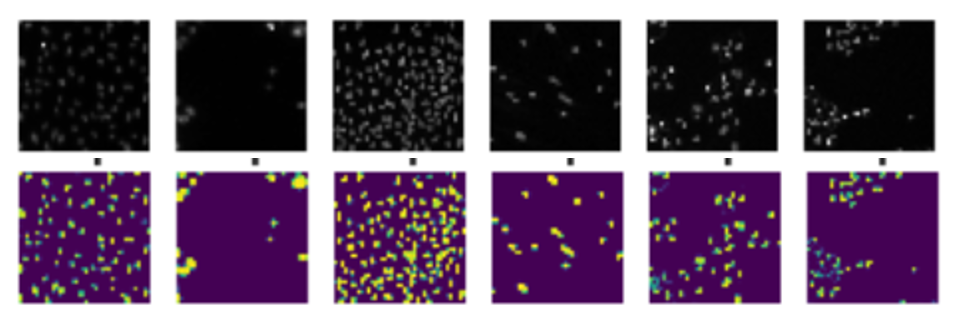
\includegraphics[scale=0.3]{figures/bce_3.png}
%		%  }
%		%     \subfig{
%		\label{Fig_bce4.sub.2}
%		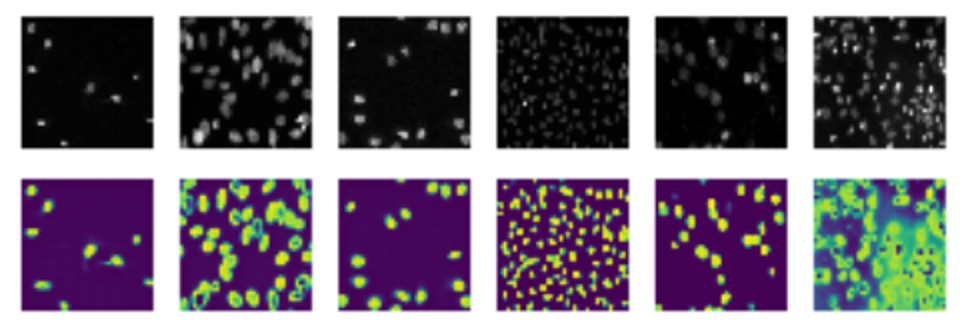
\includegraphics[scale=0.3]{figures/bce_4.png}
%		%     }
%		\caption{Training result of BCE loss function with Ir=0.001:loss=0.09 and Ir=0.0001:loss=0.15 }
%		\label{Fig_bce.main}
%		
%	\end{figure}
%	
%	
%	%%%%%%%%%%%%figure 3
%	\begin{figure}[H]
%		\centering
%		%    \subfig{
%		\label{Fig_dice3.sub.1} 
%		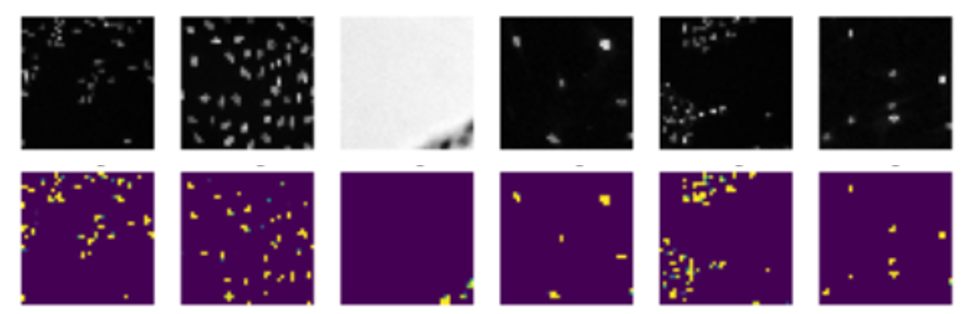
\includegraphics[scale=0.3]{figures/dice_3.png}
%		%  }
%		%     \subfig{
%		\label{Fig_dice4.sub.2}
%		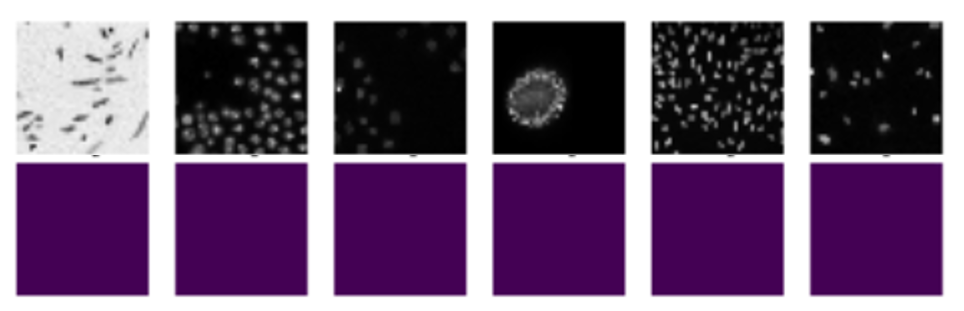
\includegraphics[scale=0.3]{figures/dice_4.png}
%		%     }
%		\caption{Training result of dice loss function with Ir=0.001:loss=0.06 and Ir=0.0001:loss=0.12}
%		\label{Fig_bce4.main}
%	\end{figure}
%	
%	%%%%%%%%%%%%figure 4
%	\begin{figure}[H]
%		\centering
%		%    \subfig{
%		\label{Fig_focal3.sub.1} 
%		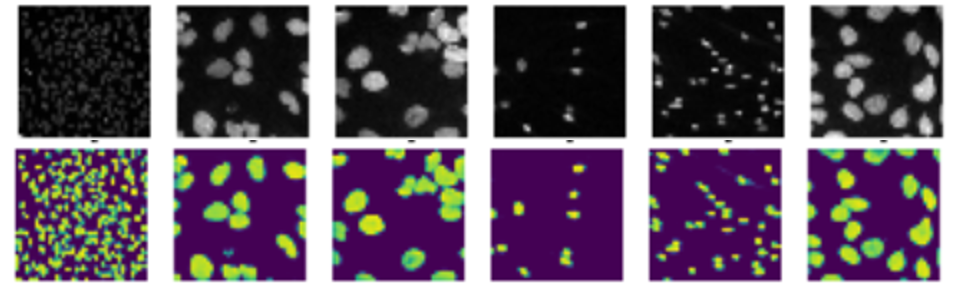
\includegraphics[scale=0.3]{figures/focal_3.png}
%		%  }
%		%     \subfig{
%		\label{Fig_focal4.sub.2}
%		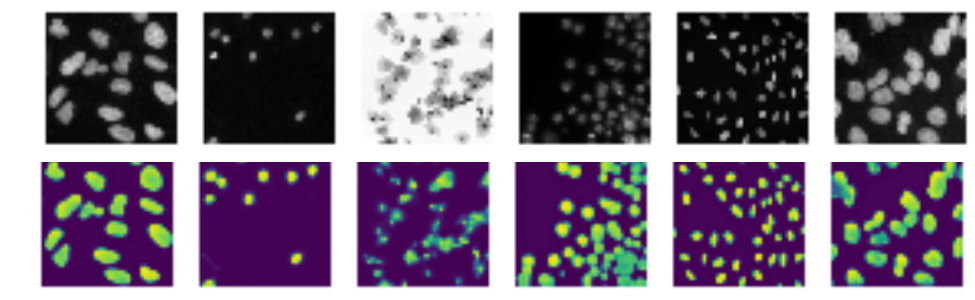
\includegraphics[scale=0.3]{figures/focal_4.png}
%		%     }
%		\caption{Training result of focal loss function with Ir=0.001:loss=0.06 and Ir=0.0001:loss=0.10}
%		\label{Fig_focl.main}
%		
%	\end{figure}
%	
%	%%%%%%%%%%%%figure 5
%	\begin{figure}[H]
%		\centering
%		%    \subfig{
%		\label{Fig_reg3.sub.1} 
%		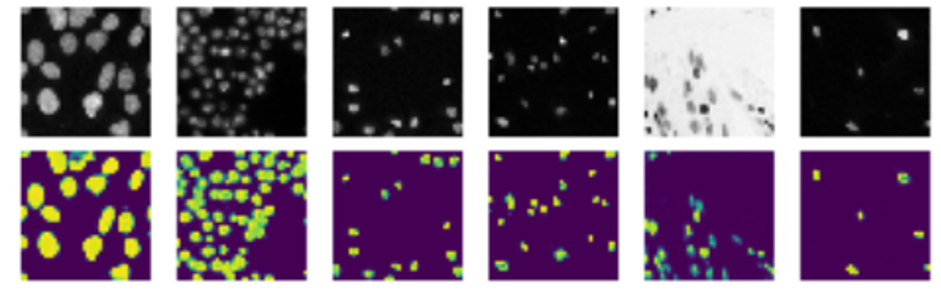
\includegraphics[scale=0.3]{figures/reg_3.png}
%		%  }
%		%     \subfig{
%		\label{Fig_reg4.sub.2}
%		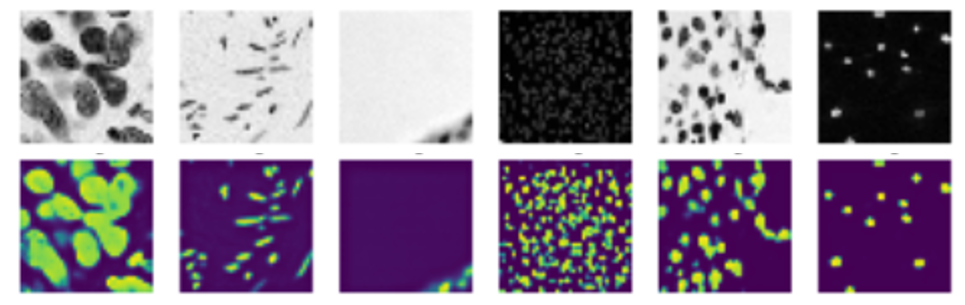
\includegraphics[scale=0.3]{figures/reg_4.png}
%		%     }
%		\caption{Training result of contiguity regularization BCE loss function with Ir=0.001:loss=0.09 and Ir=0.0001:loss=0.16}
%		\label{Fig_agi.main}
%		
%	\end{figure}
%	
%	However, that's not good enough for us. We design a new loss function which based on BCE but improved with softmax.
%	
%	%%%%%%%%%%%%figure 6
%	\begin{figure}[H]
%		\centering
%		%    \subfig{
%		\label{Fig_final.sub.1} 
%		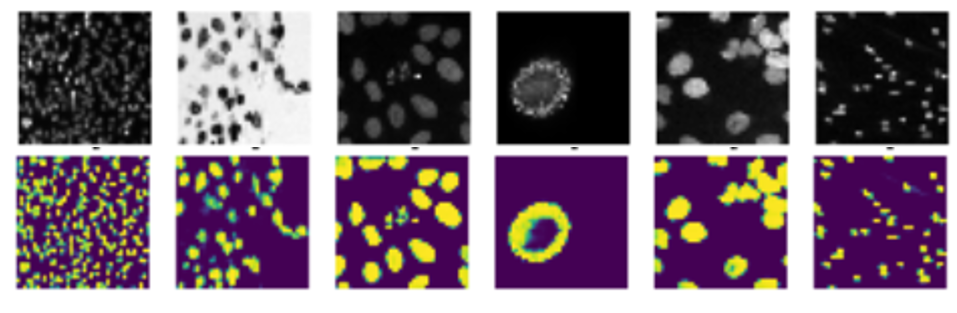
\includegraphics[scale=0.3]{figures/fin_3.png}
%		%  }
%		%     \subfig{
%		\label{Fig_final4.sub.2}
%		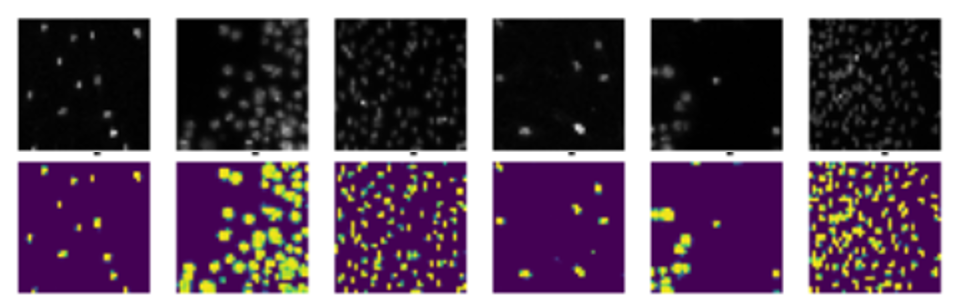
\includegraphics[scale=0.3]{figures/fin_4.png}
%		%     }
%		\caption{Training result of self designed loss function with Ir=0.001:loss=0.07 and Ir=0.0001:loss=0.06}
%		\label{Fig_agi.main}
%		
%	\end{figure}
%\end{subappendices}
%




%
% ---- Bibliography ----
%
% BibTeX users should specify bibliography style 'splncs04'.
% References will then be sorted and formatted in the correct style.
%
\bibliographystyle{splncs04}
 \bibliography{ref.bib}

\end{document}
